\section{Abstract}

Software modularization recovery algorithms automatically recognize a system's
modular structure by analyzing its implementation.
Due to the lack of well document software systems, though, the issue of testing
these algorithms is still underexplored, limiting both their adoption in the
industry and the development of better algorithms.
We propose to rely on software models to produce arbitrarily large test sets. In
this paper we consider three such models and analyze how similar the artifacts
they produce are from artifacts from real software systems.
\cite{Pollet2007}

\section{Introduction}

Development of large-scale software systems is a challenge.

A key to success is the ability to decompose a system into weakly-coupled
modules, so each module can be developed by a distinct team. Failing to do so
results in duplicated code, non-parallelism, one's work impacting another's work
etc.

The ability do modularize depends decisively on a vast knowledge about the
system, how its different parts interact to accomplish the system's goal.

Unfortunately, in the case of legacy systems, such knowledge isn't available.
Depending on its size, it might take months to understand the system so well as
to find a good modularization. XXX \cite{Parnas1972}

POR ISSO SURGIRAM software modularization recovery algorithms, also known as
software clustering algorithms or software architecture recovery algorithms. In
its most common flavor, these algorithms analyze the dependencies between
implementation components, such as classes, and then group them into modules
such as there are few dependencies between classes in distinct modules.

Software modularization recovery algorithms can, therefore, do in minutes what a
person would spend weeks or months. The question is: are the found
modularizations good? Are they similar to what a person would find? To answer
this question it's essencial to perform empirical evaluations envolving systems
with known reference modularizations.

The empirical evaluations consist of selecting a collection of systems with
known reference modularizations and then applying the algorithms to the systems.
The modularizations found by the algorithms are then compared to the reference
decompositions by a metric such as MoJo \cite{Tzerpos1999} or PrecisionRecall.

% TODO: diagram showing the evaluation of a clustering algorithm

Unfortunately there are few systems with known reference modularizations and,
because to obtain reference modularizations is costly, there are few empirical
studies, and most of them consider a couple of small and medium systems.

We therefore propose to use synthetic, i.e., computer-generated, software
dependency networks, to evaluate software modularization recovery algorithms.
These networks are generated by parametrizable models and have an embedded
reference modularizations. The goal of an algorithm is, thus, to find
modularizations that are similar to the reference modularization embedded in the
network. With this approach we can CONTAR COM a large volume of test data that
is composed of networks of different sizes and controllable characteristics.

Of course the success of this approach depends on the realism of the synthetic
networks, ie, how well they resemble networks extracted from real software
systems. In this paper we study three models and show that all of them are, by
means of a careful parameter choosing, capable of producing realistic software
networks.

The remaining sections are organized as .... Section 2, ...

%alike, resembling, exchangeable, indistiguible

\section{Software Modularization Recovery}

Aka software architecture recovery, software architecture reconstruction,
software clustering...

It's an task of reverse engineering, as defined by Tonella \cite{Tonella2007}...

%\section{Software Networks and Software Clustering}

directed graph, (un)weighted

\section{Networks Theory}

Network theory research studies general properties of many types of networks by
using statistical analysis. In the last decade, it has been found that many
networks arising from sociology, biology, technology and other domains have
remarkable similarities. It has been shown that, in these networks, the number
of vertices connected to k edges, N(k), is proportional to $k^{\-gamma}$, where
$\gamma$ is a positive constant. These networks were called scale-free networks.

Network theory has been applied to software networks and it was shown that they
are also scale-free networks \cite{Myers2003,Valverde2003}.

(in fact we can't argue the degree distribution is perfectly fit by a power law.
Anyway, the distribution is much more assymetric than normal ou Poisson's)

software indegree distribution (power law), outdegree distribution (not so power
law)

\section{Network Models}

Many models were proposed to explain the formation of scale-free networks. These
models are simple algorithms that can be proven, either formally or emprically,
to generate networks that are scale-free.


Glossary: preferential attachment

\subsection{ER (Erdos-Renyi)}

%\subsection{Configuration model}
% take the most typical software system and steal its degree sequence

\subsection{LF}

Directed weighted networks with overlapping modules.

\subsection{BCR plus}

We propose an extension to BCR model... which was proposed to model the links
between web pages.

The BCR+ model builds networks that respect a module-dependency network, that
is, a network that contains modules and allowed dependencies between modules. 
In the component dependency network, an edge between two vertices is only
allowed if there exist an edge between their respective modules.

First of all, the model generates a network that is a copy of the module
dependency network, each vertex belonging to its respective module. Then the
algorithm runs iteratively, and on each iteration it executes an operations that
modifies the network. It can add a new vertex together with an edge connecting it
to an old vertex, or it can add an edge between two existing vertices. The
choice of vertices, though, is not fully random. The probability that a
particular vertex v is choosen, P(v), is proportional to a function that involves the
in-degree or the out-degree of the node. We say that a vertex is chosen within a
set V according to a function f if

P(choose v) = f(v) / sum(v in V, f(v))

The denominator is a normalizing factor that assures that the probabilities sum
to 1.

out-neighbors(v) 
module(v)
neighbor-modules(v)

choose event with probabilities (p, q, r)
event 1:
  choose w within V according to f(x) = din + in-degree(x)
  add new vertex v to the module of w
  add edge from v to w
event 2:
  choose w within V according to f(x) = dout + out-degree(x)
  add new vertex v to the module of w
  add edge from w to v
event 3:
  choose v within V according to f(x) = dout + out-degree(x)
  choose case with probabilities (mu, 1 - mu)
  case 1: % out
    choose w within neighbor-modules(v) - neighbors(v) according to f(x) = din + in-degree(x)
    add edge from v to w
  case 2:
    choose w within module(v) - neighbors(v) according to f(x) = din + in-degree(x)
    add edge from v to w
end

picks a event that evolves
the network. Each event has an associated probability.

* Add a node with ongoing edge. With probability p, a new vertex is added to the network, together with an
edge from the new vertex to an existing vertex, chosen preferentially according
to .... Considering din = 0, this means that a vertex with indegree = 8 is
twice more likely to receive the edge than a vertex with indegree = 4. The
parameter din can be used to alleviate the handicap. (If din = 4, the first
vertex will only be 3/2 more likely to receive the edge). The new vertex is
put on the same cluster as the old vertex.

* Add a node with ingoing edge. With probability q, a new vertex is added to the network, together with an
edge from an existing vertex, chosen preferentially accordingly to dout +
outdegree, to the new vertex. The new vertex is put on the same cluster as the
old vertex. This case is similar to the previous case.

* Add an edge. With probability r, a new edge is added between two vertices, v and w. v is
chosen according to .... After that, with prob X, w is chosen from one of the
modules connected to v's module, else it's chosen from v's own module. In any
case, the exact choice is made according to ...

It's a growth model, that is, it can take as input an existing network and
evolve it.

TODO: Argument: why the imposed modules are natural modules?

\subsection{CGW}

The CGW was proposed to model the evolution of software systems organized in
modules. It was proven formally to generate scale-free networks.

The CGW model is similar to BCR+ in which it is a growth model. The initial
network is composed of two vertices with a directed edge between, belonging
to the same module. The other M - 1 modules are initially empty.

Then, at each iteration, the algorithm executes one of the following events:

* With probability p1, one vertex is added to a randomly-chosen module, together
with e1 edges from p1 to vertices chosen according to module-based preferential
attachment.

* With probability 

Accounts for the removal of edges. Growth model.

%%%%%%%%%%%%%%%%%%%%%%%%%%%%%%%%%%%%%%%%%%%%%%%%%%%%%%%%%%%%%%%%%%%%%%%%%%%%%%
%%%%%%%%%%%%%%%%%%%%%%%%%%%%%%%%%%%%%%%%%%%%%%%%%%%%%%%%%%%%%%%%%%%%%%%%%%%%%%
%%%%%%%%%%%%%%%%%%%%%%%%%%%%%%%%%%%%%%%%%%%%%%%%%%%%%%%%%%%%%%%%%%%%%%%%%%%%%%

\section{Experimental Setup}

% Is there such a thing as softwareness? Can we reproduce it?

``softwareness''

Our hypothesis is that at least one of the presented models can synthesize
networks that resemble software networks. We already know that they produce
networks that, just like software networks, are scale-free. This single
property, though, isn't enough to prove the hypothesis, since there are many
known scale-free networks extracted from many distinct domains of knowledge. It
is important to distinguish between software and non-software networks.

% v.  differentiate, differ; distinguish; contrast; discern 

The approach we chose to test our hypothesis was to build a network classifier:
an algorithm that analyses a network and classifies it as a software network or
as a non-software network. If a classifier is capable of classifying with high
accuracy both software and non-software networks, then we can apply it to
synthetic networks and see if they are discernable from software networks.
it gives a fair approximation apply it on synthetic networks. We expect that
some synthetic networks will be so similar to software networks that they will
be classified as software networks.

The experiment we conducted to evaluate the models, described in details in the
following sections, can be summarized as such:
* First of all, we collected both software and non-software networks
* Then, we devised a classifier
* After that, we applied the classifier to our data set and evaluated its
accuracy, precision and recall.
* After we came to an acceptable classifier, we synthesized many networks by
varying the parameters on the models we presented.
* Finally, we classified all synthesized networks as software or non-software.

After that we analysed the results and tried to understand which parameters
of each model contribute mostly to the softwareness of their networks

%First of all, we need a data set containg both software and non-software
%networks. 
%Therefore, in order to prove our hypothesis we must show that, according to some
%criterion, some of at least some of
%the synthetic networks are more similar to software networks than other networks
%are.
%What we are looking for, after all, is an oracle that accepts software networks
%and rejects non-software networks. If the oracle has these two properties, we
%can be confident that it'll accept only synthetic networks that resemble
%software networks.

\subsection{Real Networks Data Set}

For this experiment we have collected 65 software systems written in the Java
programming language and 66 networks from other domains, such as biology,
sociology and linguistics. Both the software systems and the networks are freely
available on the Internet.

As of this writing, Java is a popular programming language, for which there is
plenty of open source software CITE. Also, there are many dependency extractors
for this language. We have extracted the dependency network for each software
system using a tool called Dependency Finder CITE, for its easy integration with
scripts. Dependency Finder looks for dependencies by means of static analysis of
Java bytecode and outputs the dependency network in a XML file. Although this
network is in a detailed level, showing dependencies between fine-grained
implementation entities such as attributes and methods, we have abstracted it to
a network of dependencies between classes. The network is directed and
non-weighted. The size of the networks range from XXX to YYY.

% JARs?

The networks from other domains were collected in websites of complex network
research groups. The domains include sociology, linguistics, biology and
technology. The size of the networks range from XXX to YYY vertices.

\subsection{Classifier} % Software network classifier

In a recent work, Milo et al. proposed to distinguish networks of different
domains by analyzing the triad concentration of each network. A triad is simply
a network with three vertices in which all vertices are connected. There are
only 13 distinct triads -- one for each configuration of directed edges --, as
shown in Figure \ref{fig:triads}.
\cite{Milo2002}
%CONSIDERING all the possible configurations of
%directed edges between three vertices, there are to 13 triads in which all
%vertices are connected, as shown in Figure X. 

\begin{figure*}[!t]
\centering
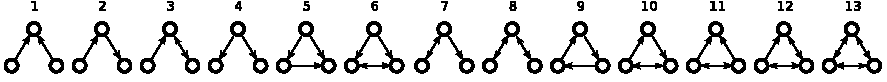
\includegraphics[width=1.0\textwidth]{triads}
\caption{Triads (id vs. graph. reprs.)}
\label{fig:triads}
\end{figure*}

In order to characterize a network, one can count how many times each of the
13 triads appear on the network. The result is a triad concentration profile.
Figure 1a show triads for a software system... Figure 2a show triads for network
from domain X. \ref{fig:profiles}

\begin{figure*}[!t]
\center
\subfigure[ref1][Software
network]{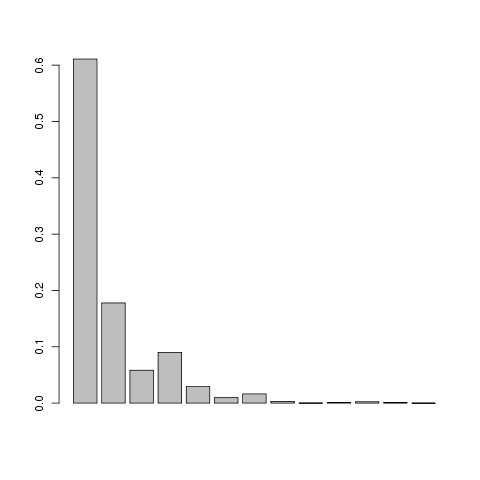
\includegraphics[width=2.5in]{triads-software}}
\hfil
\subfigure[ref2][Non-software network]{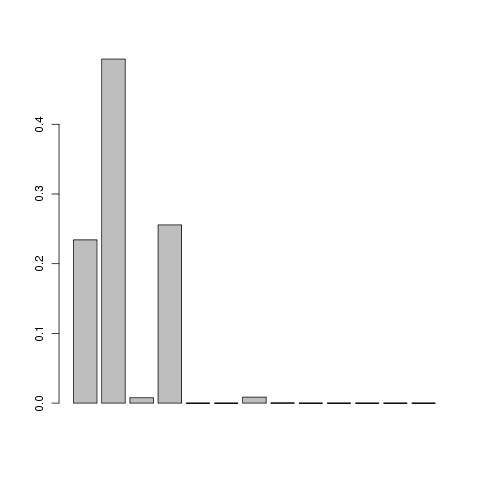
\includegraphics[width=2.5in]{triads-nonsw}%
}
\caption{Triad profiles}
\label{fig:profiles}
\end{figure*}


Then, in order to measure how similar two networks are, Milo et al computed
Pearson's correlation coefficient between the two corresponding profiles.

CITE igraph

In order two measure the softwareness of a network, we measure the correlation
between the network's profile and the profile of each of the 65 software
networks in our sample. We then compute the average of these correlations and
call it the S-score, that varies between 0 and 1. The greater the S-score, more
likely that the network is a software network.

In order to build our classifier, we need a threshold for the S-score, so
networks are classified as software networks only when they have S-score greater
or equal to this threshold. We computed the S-score for each of the 65 software
systems and found an average S-score of 0.97 with standard deviation of 0.03.
Using the three-sigma rule from statistics, we chose the threshold as 0.97 - 3 *
0.3, that is 0.88. 

The small standard deviation shows that triad concentration profiles indeed
characterize well the software domain.

\subsubsection{Classifier Validation}

In order to assess if the classifier is capable of distinguishing between
software and non-software networks, we applied it to all the networks from our
sample. 

Most software networks were classified correctly, which is not surprising since
the classifier was based on them.

Precision: X, recall: Y

Curiously, polblog had a very high S-score. This issue requires further 
investigation. Anyway, we cannot deny the possibility that it is really very
software-like.

We could have chosen another value for the threshold, and it would affect the
precision and the recall. For instance, had we chosen 0.82, we would end with
100\% recall and x\% precision. For us, though, it is more important to have a
high precision, so we keep the threshold 0.88.

We also generated networks with the ER model, which is known to generate
networks that are not scale-free and, thus, are very different from software
networks. All the ER networks were classified as non-software.

%Following Milo et al., We then used Pearson's correlation coefficient as a
%similarity measure between two networks. For each software network, we then
%computed the average correlation coefficient (ACC) to the other software
%networks. We've observed that among software networks the ACC is X +- Y.

% avg: 0.97. stdev: 0.03
%We then computed, for each non-software network, the ACC to the 65 software
%networks. By the 3-sigma rule, we use X as the threshold for realistic software
%networks: networks whose ACC is below this threshold are rejected.
%The oracle has X precision and X recall...

\subsection{Network Synthesis}

In assessing the realism of a model, we want to know if, with a proper choice of
parameters, the model is capable of producing a realistic network. In order to
do so, we must generate many networks using different combinations of
parameters. 

Since most of the parameters can assume infinite distinct values, we chose to
fix some of them and vary the others in discrete steps. In all models the number
of vertices was fixed to 1000. We generated one network for each set of
parameters. Here we describe the criteria we use to choose the parameters for
each model.

\subsubsection{BCR+}

We chose five different module dependency networks, which where extracted from
actual dependencies between modules of five different software systems of our
sample, ranging from 2 to 32 modules. The module dependency networks are shown
on Figure \ref{fig:architectures}. 

\begin{figure*}[!t]
\centering
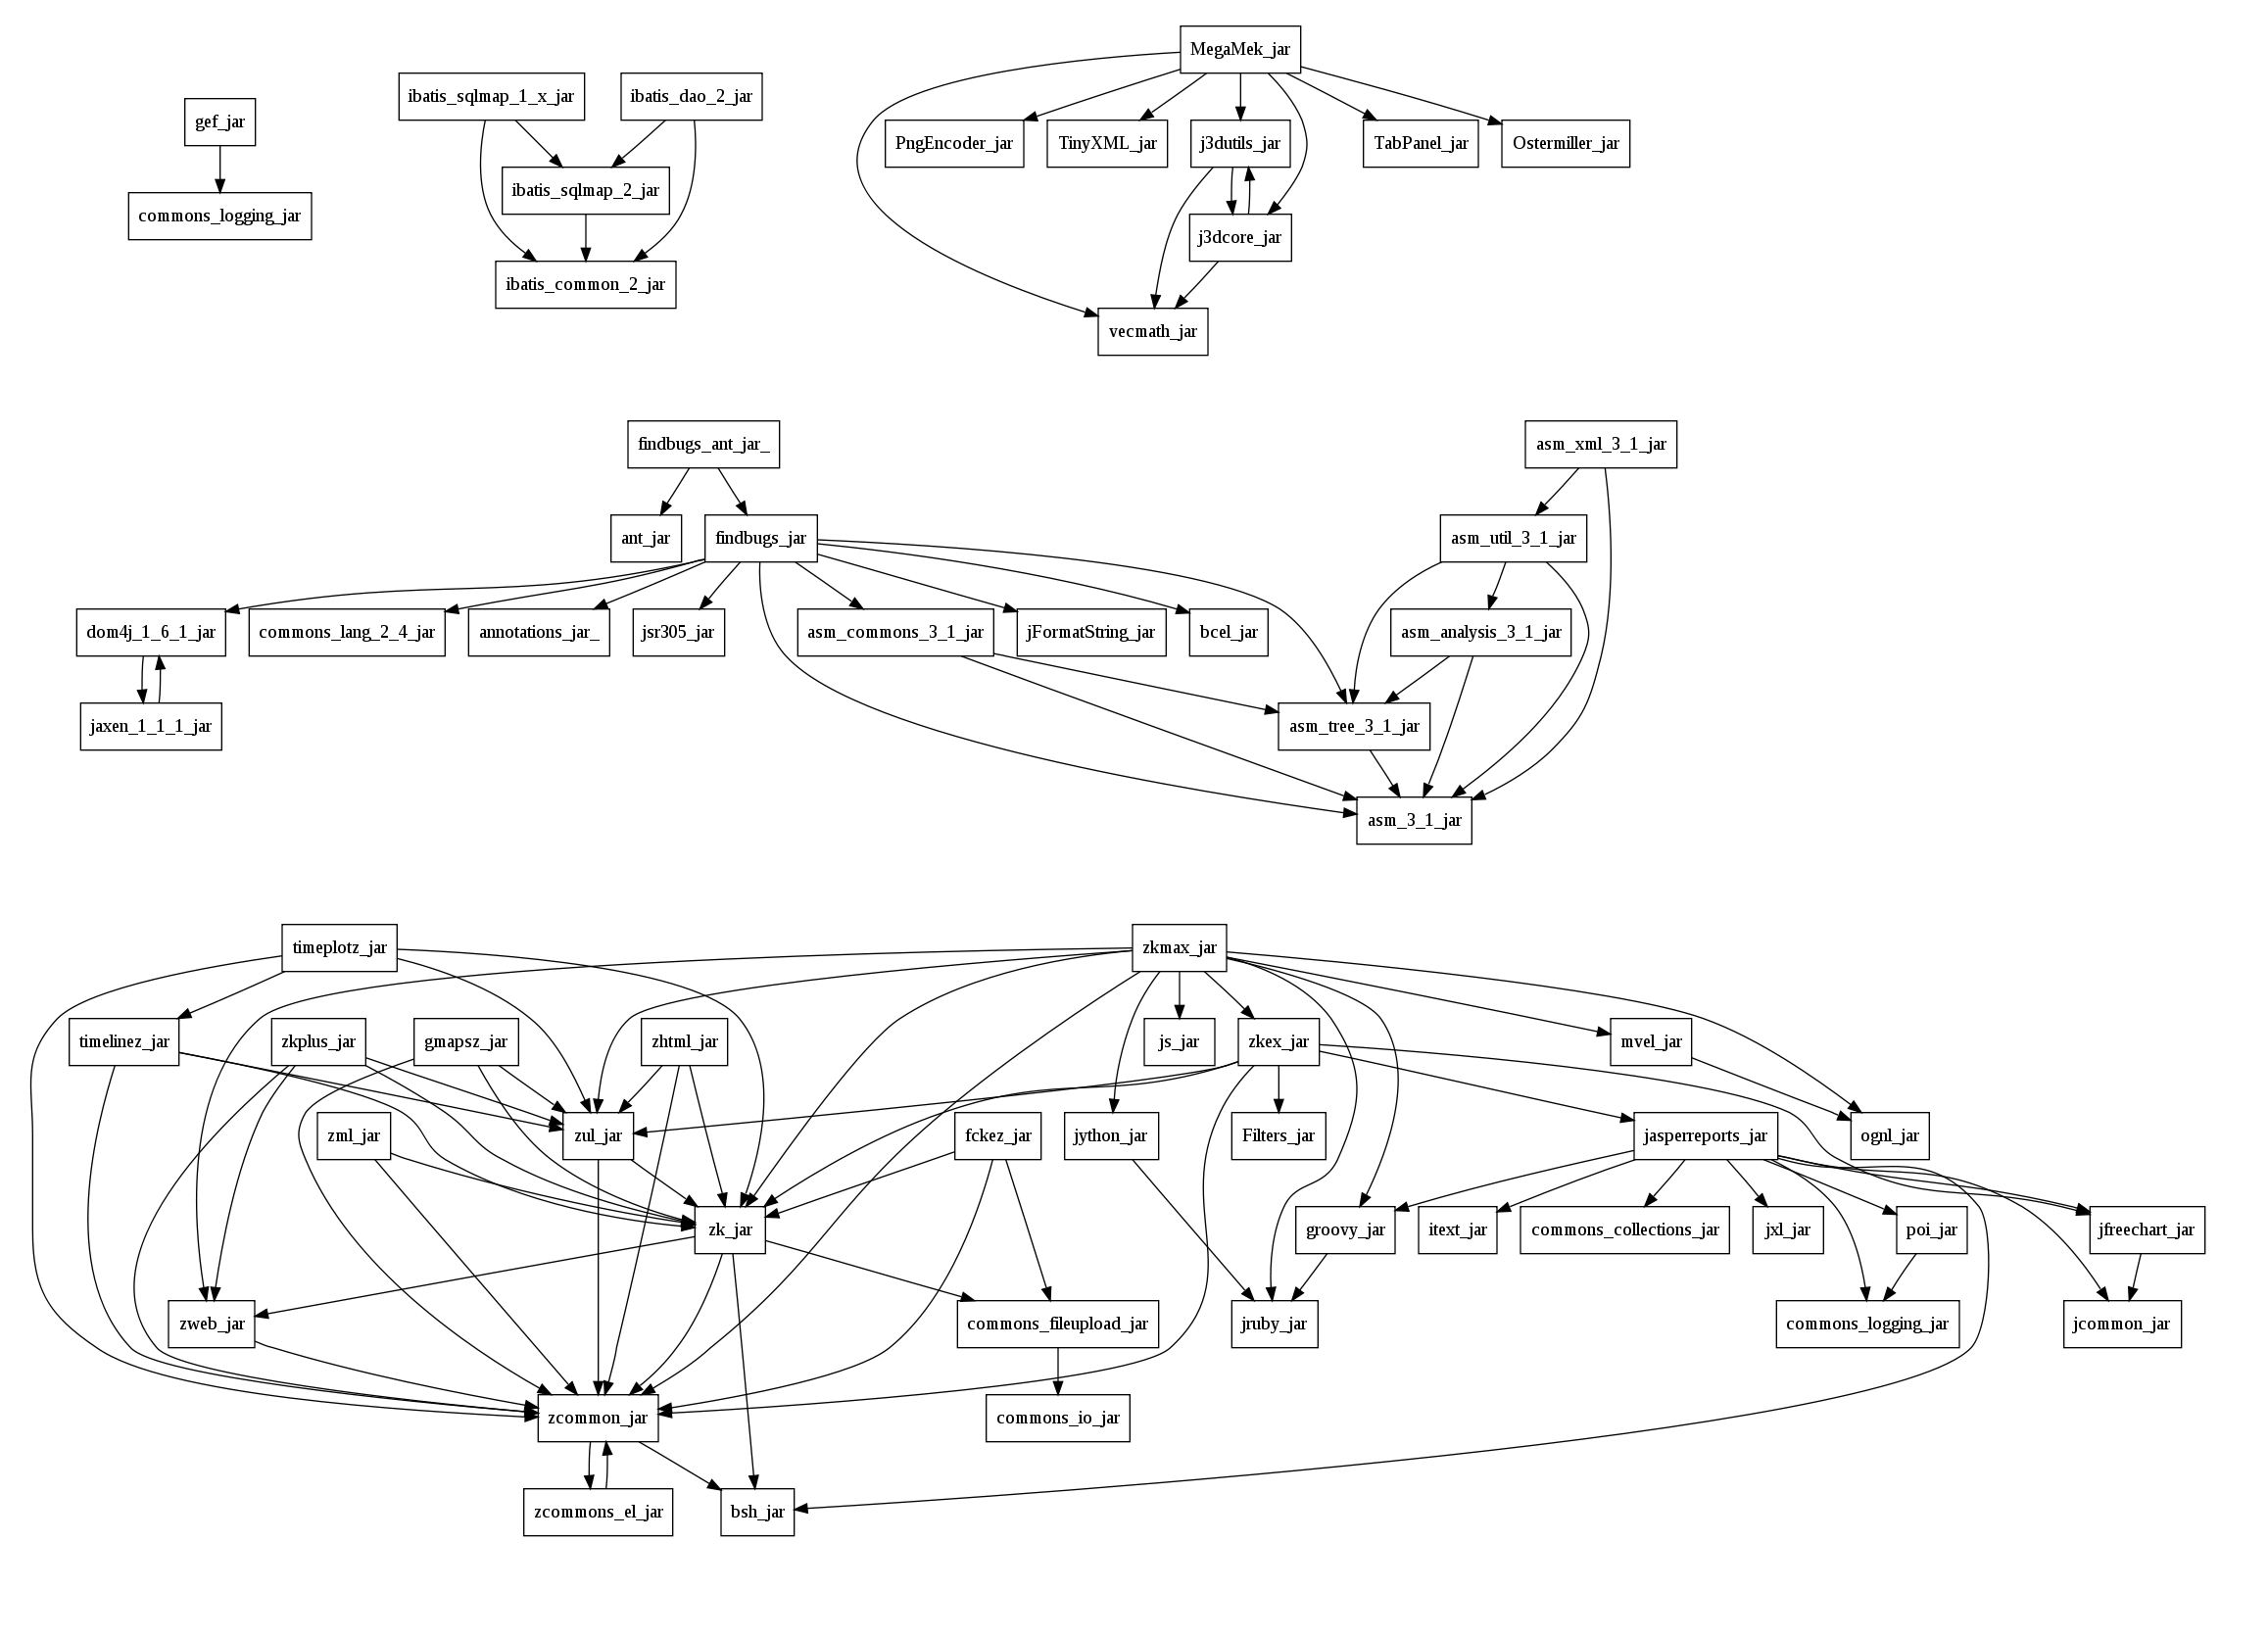
\includegraphics[width=1.0\textwidth]{architectures}
\caption{Module dependency graphs}
\label{fig:architectures}
\end{figure*}

%02-gef
%04-ibatis
%08-megamek
%16-findbugs
%32-zk

The probabilities p, q and r were given all possible values from 0.0 upto 1.0,
in 0.2 steps, such as the sum of the probabilities was 1. Since the only events
that create vertices are those associated with probabilities p and q, we imposed
the additional restriction that p + q > 0.

For deltain and deltaout we assigned the integer numbers from 0 to 4. TODO: why

Finally, we chose mu from 0.0 to 0.6 in 0.2 steps. It does not make sense to
choose higher values since they mean that there will be more edges connecting
different models.

Total: 9,500 networks.

\subsubsection{LF}

Like BCR, we choose mu ranging from 0.0 to 0.6 in 0.2 steps. For the remaining
parameters we selected values from our sample of software systems. For degexp,
..., we picked the minimum, the median and the max values.

Total: 1,296 networks

\subsubsection{CGW}

p1,p2,p3,p4 ranging from 0.0 to 1.0 in 0.2 steps, with p1 > 0, p1 + p2 + p3 + p4 = 1.0.
e1,e2,e3,e4 in 1, 2, 4, 8 (except that when pi = 0, ei is ignored).
2*p4*e4 >= p1*e1 + p2*e2, so the number of edges created is at least twice
the number of edges removed (to avoid long run times)
alpha in -1, 0, 1, 10, 100, 1000. 
m in 2, 4, 8, 16, 32 (just like bcr and lfr)

Total: 38,790 networks

\section{Softwareness Evaluation}

We used our classifier ...

Table: Model | Number of Networks | Realistic Networks | Percent \%

Show some graphs: histogram of average correlations for each model.
\ref{fig:histograms}


\begin{figure*}[!t]
\center

\subfigure[Software network]{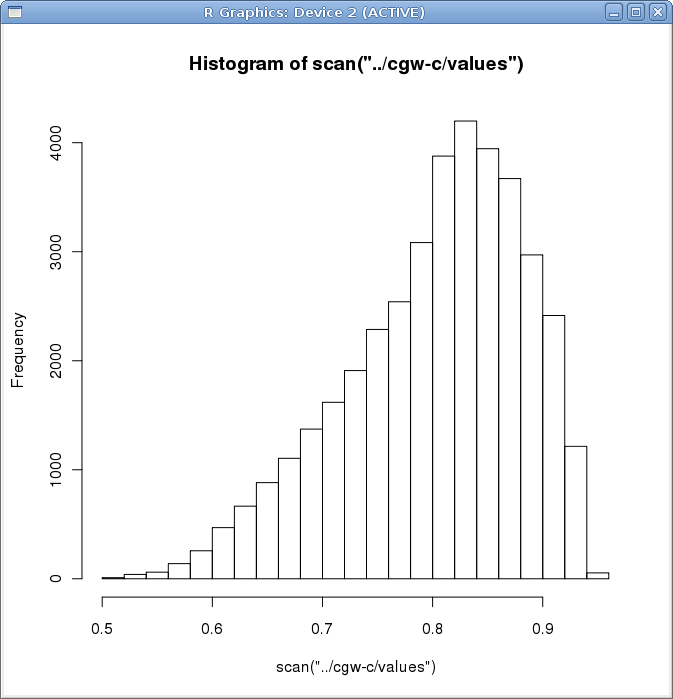
\includegraphics[width=1.0in]{hist-cgw}}

\subfigure[Non-software network]{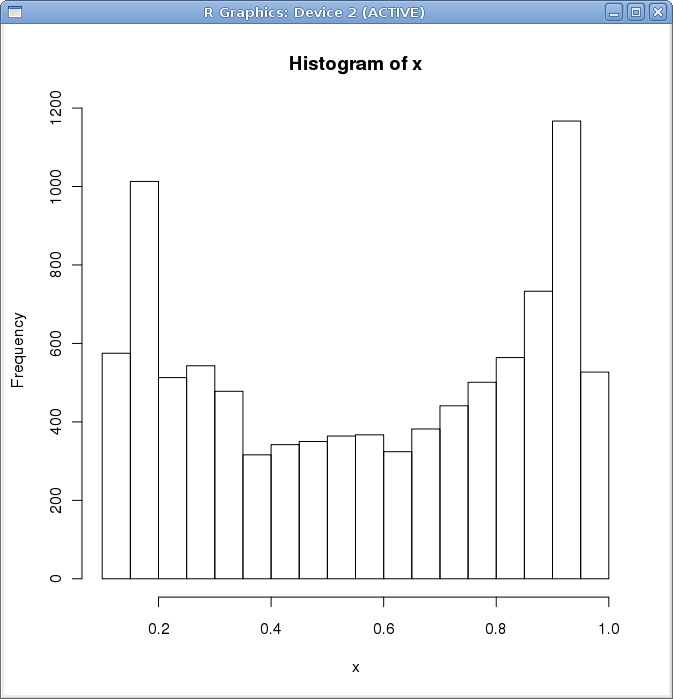
\includegraphics[width=1.0in]{hist-bcr}}

\subfigure[Non-software network]{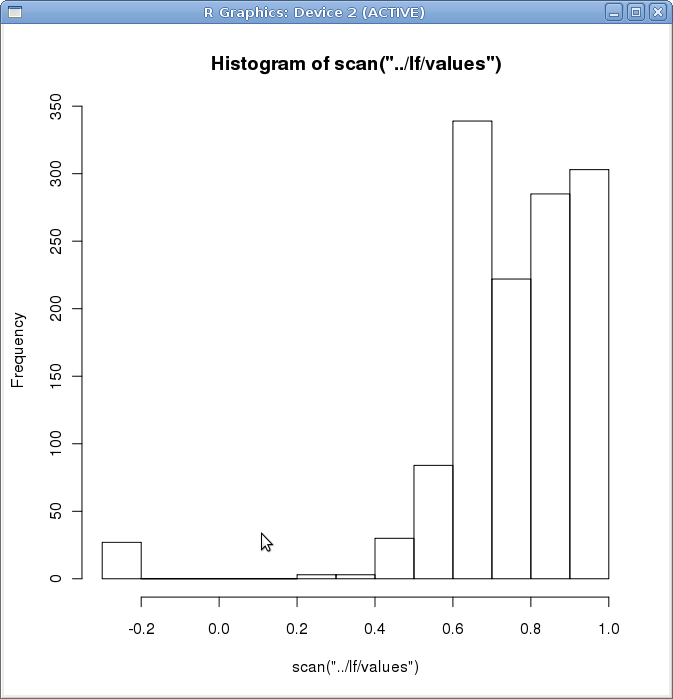
\includegraphics[width=1.0in]{hist-lf}}

\caption{Triad profiles}
\label{fig:histograms}
\end{figure*}

All models produce networks that resemble software networks.  For some
parameters, though, the networks are not realistic.

\subsection{Patterns in Parameters}

1R

Naive Bayes

\subsection{Homogeinity}

Pick realistic networks from a model. Are they similar to each other? (see
standard deviation) In other words: do the parameters make a difference?

Are they similar to networks generated by the other models? In other words: are
the models equivalent?

\section{Threats to validity}

% External validity (EV): can it be generalized?
Structural information isn't enough for a expert do produce a
decomposition (s/he may use data such as names and external documentation). 

Even when considering only structural information, is it true
that experts would find a decomposition similar to the reference decomposition
imposed by the model?

We generated only one network for each set of parameters. (as we've shown, some
parameters are redundant as they do not change significantly the realism)

Some clustering algorithms use weights and they weren't studied here.

EV: We've only studied 65 systems, which is not that much.

We only studied object-oriented systems implemented in Java. Maybe the results
would be different if we studied systems implement in other languagens or using
other paradigms. The choice of a particular technique for extracting
dependencies (static analysis) may also have impact on the structure of the
networks.

% Koschke says that experts decompositions vary by no more than 80? percent.

\section{Conclusion and Future Work}

We have shown empirically that network models found in the literature can
produce synthetic networks that are similar to the network of dependencies
between classes in object-oriented systems. This result supports the use of
synthetic networks in the evaluation of software modularization algorithms.
%that operate on class dependency networks. 

% review
The use of synthetic data is common in distributed computing research, but still
underexplored in software engineering research. Since many reverse engineering
tasks extract from component dependencies information useful for the maintenance
of a software system, we expect this work to have impact beyond the software
modularization recovery community.

%Although the use of models and synthetic data is somewhat common in distributed
%computing research, it is underexplored in software engineering research. We
%expect this work to contribute to explore t
%common in distributed computing research, simulation is underexplored
%in software engineering. This work opens a door to the usage of simulation in
%the field of reverse engineering of software in order to evaluate RE 
%algorithms.

We accept that it is very important to test the algorithms with networks
extracted from real software systems, but we argue that the use of synthetic
networks in a complementary manner can give researchers new insights about the
algorithms. First, the use of models allows the creation of large test sets,
thus diminishing the small sample effects. Moreover, the networks are created in
a controlled way, accordingly to model parameters, so it is possible to study
the behavior of the algorithms with different parameter values.

In a future work, we intend to evaluate with synthetic networks some software
clustering algorithms that were previously studied with real data. We will,
then, be able to compare the results obtained by both approaches. \cite{Wu2005}

\section{Appendix A: list of networks}

Software networks:

From SourceForge:
AbaGuiBuilder-1.8
alfresco-labs-deployment-3Stable
aoi272
stendhal-0.74
battlefieldjava-0.1
checkstyle-5.0
dom4j-1.6.1
findbugs-1.3.8
freetts-1.2.2-bin
ganttproject-2.0.9
geoserver-2.0-beta1-bin
geotools-2.5.5-bin
gfp\_0.8.1
hibernate-distribution-3.3.1.GA-dist
hsqldb\_1\_8\_0\_10
iBATIS\_DBL-2.1.5.582
iReport-nb-3.5.1
JabRef-2.5b2-src
jailer\_2.9.9
jalopy-1.5rc3
jasperreports-3.5.2-project
jfreechart-1.0.13
pentaho-reporting-engine-classic-0.8.9.11
jGnash-2.2.0
jgraphpad-5.10.0.2
jmsn-0.9.9b2
juel-2.1.2
JXv3.2rc2deploy
makagiga-3.4
MegaMek-v0.34.3
iFreeBudget-2.0.9
mondrian-3.1.1.12687
oddjob-0.26.0
openxava-3.1.2
pdfsam-1.1.3-out
pjirc\_2\_2\_1\_bin
pmd-bin-4.2.5
proguard4.3
smc\_6\_0\_0
squirrel-sql-3.0.1-base
squirrel-sql-3.0.1-standard
tvbrowser-2.7.3-bin
villonanny-2.3.0.b02.bin
rapidminer-4.4-community
zk-bin-3.6.1

From other places:

ArgoUML-0.28
GEF-0.13-bin
Hl7Comm.1.0.1
IRPF2009v1.1
broker-4.1.5
dbwrench
ec2-api-tools
ermodeller-1.9.2-binary
flyingsaucer-R8
gdata-src.java-1.31.1
guice-2.0
gwt-windows-1.6.4
jai-1\_1\_4-pre-dr-b03-lib-linux-i586-08\_Jun\_2009
jakarta-tomcat-5.0.28-embed
juxy-0.8
myjgui\_0.6.6
peer-4.1.5
subethasmtp-3.1
thinkui\_sqlclient-1.1.2
worker-4.1.5

Other networks:

3 circuit networks (circuit-s208 circuit-s420 circuit-s838)

5 facebook networks (facebook-Caltech36 facebook-Georgetown facebook-Oklahoma
facebook-Princeton facebook-UNC28)

5 language networks (lang-english  lang-french lang-japanese lang-spanish)

43 metabolic networks

polblogs

3 protein networks (protein-a4j protein-AOR protein-eaw)

2 social networks (social-leader social-prison)

other networks:

yeast

beta3sreduced
celegansneural

czech
ecoli-metabolic
